\documentclass{beamer}
\mode<presentation>{
	\usetheme{Madrid}
}

\usepackage{graphicx}
\usepackage{algorithm}
\usepackage{algpseudocode}
\usepackage{booktabs}

\usepackage{tikz}
\usepackage{amsmath}
\usetikzlibrary{matrix}

\title[University of Connecticut] {Hidden Markov Models in Biological Sequence Analysis}

\author{Huyen D. Nguyen}

\institute[]{University of Connecticut \\
	\medskip
	\text{Department of Statistics}\\
}
\date{November 06, 2023}

\begin{document}
\begin{frame}
	\titlepage
\end{frame}

\begin{frame}{Introduction: Hidden Markov Model}
	\begin{itemize}
		\item A \textbf{hidden Markov Model (HMM)} is a statistical model that can be used to describe the evolution of observable events that depend on a Markov process with unobservable states. 
		\item Many real world problems deal with classifying raw observations into a number of categories or class labels that are more meaningful.
		\item HMM applications in signal processing, pattern recognition, economics, finance, bioinformatics, etc.
	\end{itemize}
\end{frame}

\begin{frame}{Introduction: Biological Sequence Analysis}
	\begin{itemize}
		\item The modeling approach of HMM is useful in modeling biological sequencess.
		\item Example: Proteins generally consists of multiple domains \cite{yoon2009hidden}. 
		\begin{enumerate}
			\item Predict the constituting domains (one or more hidden Markov states) and their location in amino acid sequences (observations).
			\item Find the protein family that the a protein sequence belongs.
		\end{enumerate}
	\end{itemize}
\end{frame}

\begin{frame}{Outline}
	\tableofcontents
\end{frame}

\section{Overview of Hidden Markov Model}
\begin{frame}{HMM Definition}
	\begin{itemize}
		\item Observed symbols (events/states): $X_1, X_2, ..., X_L$.
		\begin{itemize}
			\item Each symbol $X_n$ can take on a value from the set $\textbf{O} = \{ O_1,..., O_N\}$.
		\end{itemize}
		\item Unobserved state: $Y_n, Y_2,...Y_L$.
		\begin{itemize}
			\item Each state $Y_i$ can take on a value from the set $\textbf{S} = \{S_1, S_2,...S_M\}$.
		\end{itemize}
		\item Initial state probability $\pi(i)$, $i \in S$
		\begin{equation}
			\pi(i) = P(Y_1 = i).
		\end{equation}
	\end{itemize}
\end{frame}

\begin{frame}{HMM Definition}
	\begin{itemize}
		\item Transition probability $t(i,j)$: the probability of moving from state $i$ to $j$, $i,j \in \textbf{S}$
		\begin{equation}
			\begin{split}
				t(i,j) & = P(Y_{n+1} = j \vert Y_n = i, Y_{n-1} = i_{n-1},\cdots, Y_1 = i_1) \\
				& = P(Y_{n+1} = j \vert Y_n = i).
			\end{split}
		\end{equation}
		\item Emission probability $e(x,i)$: the probability of observing $X_n = x$ when the hidden state is in state $i$, $x \in \textbf{O}$ and $i \in \textbf{S}$
		\begin{equation}
			\begin{split}
				e(x, i)
				& = P(X_n = x \vert Y_n = i) .
			\end{split}
		\end{equation}
	\end{itemize}
	\begin{figure}
		\centering
		\resizebox{3in}{!}{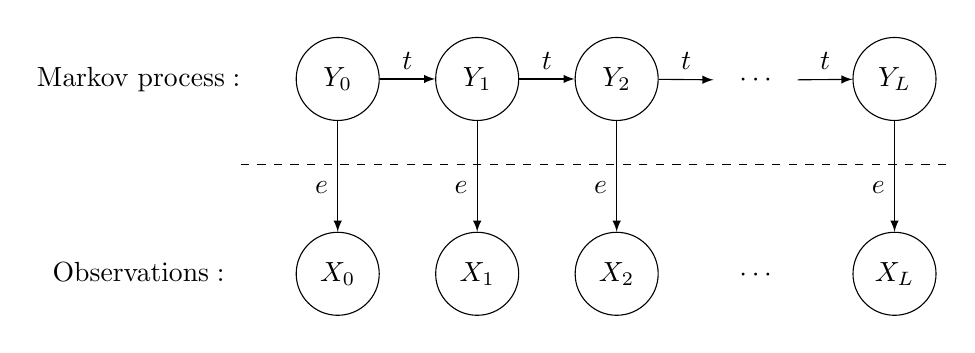
\begin{tikzpicture}
				\matrix[matrix of math nodes,column sep=2em,row
				sep=4em,cells={nodes={circle,draw,minimum width=3em,inner sep=0pt}},
				column 1/.style={nodes={rectangle,draw=none}},
				column 5/.style={nodes={rectangle,draw=none}},
				ampersand replacement=\&] (m) {
					\text{Markov process}: \&
					Y_0 \& Y_1 \& Y_2 \& \cdots \& Y_{L}\\
					\text{Observations}: \& 
					X_0 \& X_1 \& X_2 \& \cdots \& X_{L}\\
				};
				\foreach \X in {2,3,4,5}
				{\draw[-latex] (m-1-\X) -- (m-1-\the\numexpr\X+1) node[midway,above]{$t$};
					\ifnum\X=5
					\draw[-latex] (m-1-6) -- (m-2-6) node[pos=0.6,left]{$e$};
					\else
					\draw[-latex] (m-1-\X) -- (m-2-\X) node[pos=0.6,left]{$e$};
					\fi}
				\draw[dashed] ([yshift=1ex]m.east) -- ([yshift=1ex]m.east-|m-1-1.east);
		\end{tikzpicture}}
		\caption{An example of a hidden Markov model.}
		\label{fig:HiddenMarkov}
	\end{figure}
\end{frame}
\section{The Scoring Problem and the Forward Algorithm}
\section{The Decoding Problem and the Viberti Algorithm}
\begin{frame}{Decoding Problem: CG island example}
	\begin{itemize}
		\item In genome, the frequency of CG dinucleotide is relative low (about 1\% in human genome) because of methylation. 
		\item The resulting methylated cytosine has the tendency to further deaminate into thymine \cite{compeau2018bioinformatics}.
		\item However, mythelation is often suppressed around genes, particularly near transcriptional start sites.
		\item These areas are called CG islands, where CG appears relatively frequently compared to the rest of the genome.
		\item Identifying CG islands is useful in identifying different genes.
	\end{itemize}
\end{frame}

\begin{frame}{HMM for Decoding Problem}
	\begin{itemize}
		\item CG Island Decoding Problem: Given an RNA sequence, we want to identify the high CG content region and low CG content region.
		\item HMM for Decoding Problem: Given a symbol sequence \textbf{X}, find optimal state sequence or optimal path in the HMM that maximizes the observation probability of the given sequence.
	\end{itemize}
\end{frame}

\begin{frame}{HMM for Decoding Problem}
	Example 1 \cite{borodovsky2006problems}: Consider the sequence S = \textbf{GGCACTGAA} and the initial, transition, and emission probability as in the following graph
	\begin{figure}
		\centering
		\includegraphics[width = 0.7\textwidth]{example1.png}
		\label{fig:example1}
		\caption{Example of HMM for CG island problem: 2 hidden Markov states H (high CG content) and L (low CG content), 4 observable symbols A,T C,G.}
	\end{figure}
\end{frame} 
\begin{frame}{Viberti Algorithm}
	\begin{itemize}
		\item Viberti Algorithm is a dynamical programming algorithm that computes the most probable path recursively.
		\item Define the probability of the most probable path ending with state $n$ at $i$ with $i \in \textbf{S}$
		\begin{equation}
			\gamma(n, i) = \max_{y_1\cdots y_{n-1}} P(x_1\cdots x_n, y_1\cdots y_{n-1} y_n = i).
		\end{equation}
		\item Compute it recursively it using the formula
		\begin{equation}
			\gamma(n, i) = \max_k[\gamma(n-1,k) t(k,i) e(x_n, i)].
		\end{equation}
		\item The opimal path can be found by tracing back the recusions that led to the maximum probability.
	\end{itemize}
\end{frame}

\begin{frame}{Viberti Algorithm}
	Back to example 1: The most probable path (sequence of hidden states) is \textbf{HHHLLLLLL} and its probability is $2^{-24.49} = 4.25 \times 10^{-8}$.
	\begin{figure}
		\centering
		\includegraphics[width = 0.7\textwidth]{example1cal.png}
		\label{fig:example2cal}
		\caption{Viberti algorithm calculation for example 1 using $\log_2$ and back tracing to find the most probable path.}
	\end{figure}
\end{frame}

\section{The Training Problem and the Baum-Welch algorithm}
\section{Extensions of HMM for Biological Sequence Analysis}
\begin{frame}{References}
	\bibliographystyle{acm}
	\bibliography{refs}
\end{frame}

\end{document}